\section{Overview}
\label{sec:overview}

As stated in \cref{ssec:goals}, one of the design goals during the project was
to keep the implementation of the REPL IDE-agnostic. To achieve this goal, the
product has been split into a backend and several frontends. This backend
interacts with the Spoofax services on behalf of the frontends. An overview of
its design can be found in \cref{fig:uml-overview}. To request and receive
results from the backend, every frontend should at least implement the
\texttt{IResultVisitor} interface in the \texttt{client} package and
acquire an instance of a class implementing the \texttt{ICommandInvoker}
interface.

The \texttt{ICommandInvoker} instance maintains a map from command names to
corresponding \texttt{IReplCommand} instances. A frontend can thus send
input directly to the \texttt{execute} method, after which the command
corresponding to the input is resolved and executed. The executed command
then returns an instance of a class implementing the \texttt{IResult}
interface. The actual type of the returned class depends on the executed command
and whether the command was successful or not. The frontend is itself
responsible for deciding how to present the result types to the user.

\begin{figure}[h!]
  \centering
  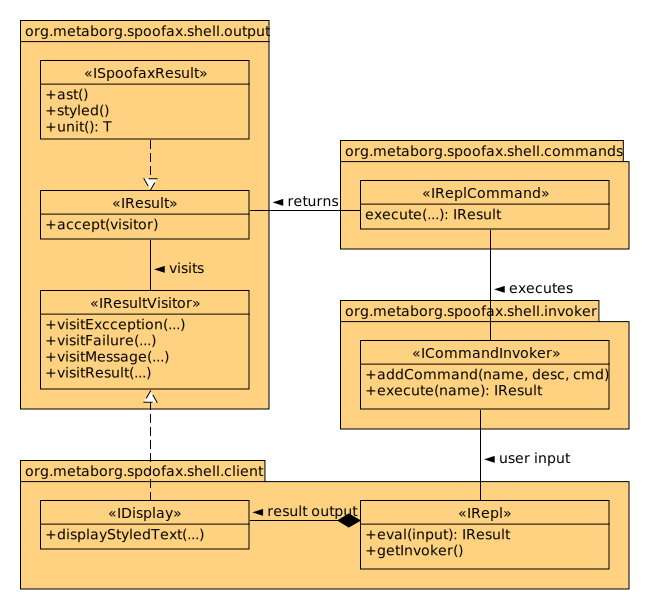
\includegraphics[width=0.75\textwidth]{uml-overview}
  \caption{An overview of the most relevant components of the backend.}
  \label{fig:uml-overview}
\end{figure}
